\documentclass[tikz,border=2pt,11pt]{standalone}
\usetikzlibrary{positioning}
\usetikzlibrary{arrows.meta}
\usepackage{amsmath}
\usepackage{amssymb}
\usepackage{tikz}
\usepackage{xcolor}
\def\@captype{figure}
\DeclareMathOperator{\Hom}{Hom}
\DeclareMathOperator{\Mod}{Mod}
\DeclareMathOperator{\sk}{sk}
\DeclareMathOperator*{\colim}{colim}
\newcommand{\id}{\mathrm{id}}
\newcommand{\sSet}{\mathbf{sSet}}
\newcommand{\Spaces}{\mathbf{Spaces}}
\newcommand{\op}{\mathrm{op}}
\newcommand{\LL}{\mathbf L}
\begin{document}
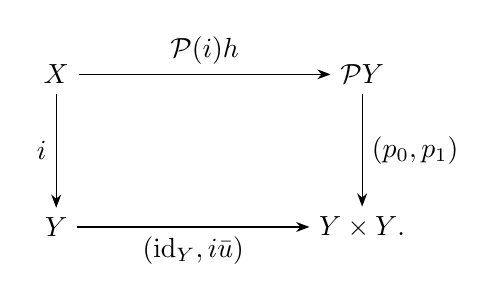
\begin{tikzpicture}[baseline=(current bounding box.center),
                   node distance=1.45cm and 3.2cm,>=Stealth]
\node (a) {\(X\)};
\node (b) [right=of a] {\(\mathcal P Y\)};
\node (c) [below=of a] {\(Y\)};
\node (d) at (b |- c) {\(Y\times Y\).};
\draw[->] (a) -- node[above] {\(\mathcal P(i)h\)} (b);
\draw[->] (a) -- node[left] {\(i\)} (c);
\draw[->] (b) -- node[right] {\((p_0,p_1)\)} (d);
\draw[->] (c) -- node[below] {\((\id_Y,i\bar u)\)} (d);
\end{tikzpicture}
\end{document}
